\documentclass{beamer}
\mode<presentation>
\usepackage{amsmath,amssymb,mathtools}
\usepackage{textcomp}
\usepackage{gensymb}
\usepackage{adjustbox}
\usepackage{subcaption}
\usepackage{enumitem}
\usepackage{multicol}
\usepackage{listings}
\usepackage{url}
\usepackage{graphicx} % <-- needed for images
\def\UrlBreaks{\do\/\do-}

\usetheme{Boadilla}
\usecolortheme{lily}
\setbeamertemplate{footline}{
  \leavevmode%
  \hbox{%
  \begin{beamercolorbox}[wd=\paperwidth,ht=2ex,dp=1ex,right]{author in head/foot}%
    \insertframenumber{} / \inserttotalframenumber\hspace*{2ex}
  \end{beamercolorbox}}%
  \vskip0pt%
}
\setbeamertemplate{navigation symbols}{}

\lstset{
  frame=single,
  breaklines=true,
  columns=fullflexible,
  basicstyle=\ttfamily\tiny   % tiny font so code fits
}

\numberwithin{equation}{section}

% ---- your macros ----
\providecommand{\nCr}[2]{\,^{#1}C_{#2}}
\providecommand{\nPr}[2]{\,^{#1}P_{#2}}
\providecommand{\mbf}{\mathbf}
\providecommand{\pr}[1]{\ensuremath{\Pr\left(#1\right)}}
\providecommand{\qfunc}[1]{\ensuremath{Q\left(#1\right)}}
\providecommand{\sbrak}[1]{\ensuremath{{}\left[#1\right]}}
\providecommand{\lsbrak}[1]{\ensuremath{{}\left[#1\right.}}
\providecommand{\rsbrak}[1]{\ensuremath{\left.#1\right]}}
\providecommand{\brak}[1]{\ensuremath{\left(#1\right)}}
\providecommand{\lbrak}[1]{\ensuremath{\left(#1\right.}}
\providecommand{\rbrak}[1]{\ensuremath{\left.#1\right)}}
\providecommand{\cbrak}[1]{\ensuremath{\left\{#1\right\}}}
\providecommand{\lcbrak}[1]{\ensuremath{\left\{#1\right.}}
\providecommand{\rcbrak}[1]{\ensuremath{\left.#1\right\}}}
\theoremstyle{remark}
\newtheorem{rem}{Remark}
\newcommand{\sgn}{\mathop{\mathrm{sgn}}}
\providecommand{\abs}[1]{\left\vert#1\right\vert}
\providecommand{\res}[1]{\Res\displaylimits_{#1}}
\providecommand{\norm}[1]{\lVert#1\rVert}
\providecommand{\mtx}[1]{\mathbf{#1}}
\providecommand{\mean}[1]{E\left[ #1 \right]}
\providecommand{\fourier}{\overset{\mathcal{F}}{ \rightleftharpoons}}
\providecommand{\system}{\overset{\mathcal{H}}{ \longleftrightarrow}}
\providecommand{\dec}[2]{\ensuremath{\overset{#1}{\underset{#2}{\gtrless}}}}
\newcommand{\myvec}[1]{\ensuremath{\begin{pmatrix}#1\end{pmatrix}}}
\let\vec\mathbf

\title{MatGeo Presentation - Problem 1.6.14}
\author{EE25BTECH11064 - Yojit Manral}
\date{}

\begin{document}

\frame{\titlepage}
\begin{frame}{Question}
Points $\Vec{A}$$\brak{3,1}$, $\Vec{B}$$\brak{12,-2}$ and $\Vec{C}$$\brak{0,2}$ cannot be the vertices of a triangle.
\end{frame}

\begin{frame}{Solution}
\textbf{Solution:}\\
\begin{table}[h!]    
  \centering
  \begin{tabular}[12pt]{ |c| c|}
    \hline
    \textbf{Points} & \textbf{Name}\\ 
    \hline
	\myvec{7\\10} & Point $\Vec{A}$ \\
    \hline 
	\myvec{-2\\5} & Point $\Vec{B}$\\
    \hline
	\myvec{3\\4} & Point $\Vec{C}$\\
    \hline
\end{tabular}
  \caption{List of Points}
  \label{Table_1}
\end{table}\\

$\rightarrow$ Any 3 points form a triangle if the rank of co-linearity matrix is not equal to 1, in which case they become collinear. For the rank of a matrix to be 1, the number of rows with non-zero entries should be 1 in row echelon form. \\

\end{frame}

\begin{frame}{Solution}
$\rightarrow$ The co-linearity matrix is given by,

\begin{align}
\myvec{\vec{B}-\vec{A} & \vec{C}-\vec{A}}^T = \myvec{9 & -3 \\ -3 & 1}\\
\notag
\end{align}
\begin{align}
\myvec{9 & -3 \\ -3 & 1}
&\xrightarrow{R_2 \leftrightarrow R_1 + 3R_2}
\myvec{9 & -3 \\ 0 & 0}\\
\notag
\end{align}
\end{frame}

\begin{frame}{Solution}
$\rightarrow$ The above matrix is in the row echelon form. Rank of the matrix in echelon form is the number of non-zero rows. Hence, rank of the above matrix is 1.\\
$\implies$ The given 3 points A, B, C are collinear. Thus, they cannot be part of a triangle.
\begin{figure}[h!]
   \centering
   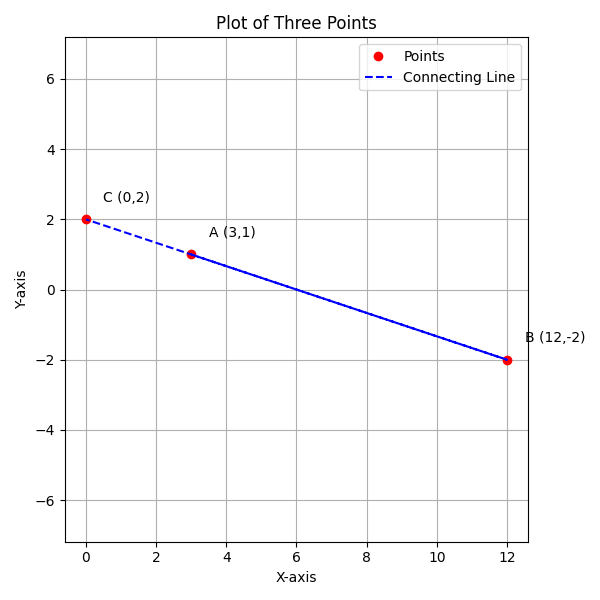
\includegraphics[width=0.4\linewidth]{figs/01.png}
   \caption{Plot of the points A, B, C}
   \label{Plot_1}
\end{figure}
\end{frame}
 % --------- CODE APPENDIX ---------
\section*{Appendix: Code}

% C program
\begin{frame}[fragile]{File: points.c}
\begin{lstlisting}[language=C]
#include <stdio.h>

int main() {
  FILE *fp;

  // -------------------
  // Question 1.6.14
  // -------------------


  fp = fopen("points.dat", "w");
  fprintf(fp, "%d,%d,%d\n", 3, 1, 0);  // A
  fprintf(fp, "%d,%d,%d\n", 12, -2, 0);   // B
  fprintf(fp, "%d,%d,%d\n", 0, 2, 0); // C
  fclose(fp);
  return 0;
  }
\end{lstlisting}
\end{frame}

% Python calling C
\begin{frame}[fragile]{File: call\_c.py}
\begin{lstlisting}[language=Python]
import subprocess

# Compile the C program
subprocess.run(["gcc", "points.c", "-o", "points"])

# Run the compiled C program
result = subprocess.run(["./points"], capture_output=True, text=True)

# Print the output from the C program
print(result.stdout)
\end{lstlisting}
\end{frame}

% Python plotting
\begin{frame}[fragile]{File: plot.py}
\begin{lstlisting}[language=Python]
import numpy as np
import matplotlib.pyplot as plt

# Define the points
points = np.array([
    [3, 1],     # A
    [12, -2],   # B
    [0, 2]      # C
])

# Extract x and y coordinates
x = points[:, 0]
y = points[:, 1]

# Plot the points
plt.figure(figsize=(6, 6))
plt.plot(x, y, 'ro', label='Points')           # Red dots
plt.plot(x, y, 'b--', label='Connecting Line') # Dashed blue line

# Annotate each point
labels = ['A (3,1)', 'B (12,-2)', 'C (0,2)']
for i in range(len(labels)):
    plt.text(x[i] + 0.5, y[i] + 0.5, labels[i], fontsize=10)

# Add plot details
plt.title('Plot of Three Points')
plt.xlabel('X-axis')
plt.ylabel('Y-axis')
plt.grid(True)
plt.axis('equal')
plt.legend()
plt.tight_layout()
plt.show()
\end{lstlisting}
\end{frame}

\end{document}
